\begin{table*}[ht!]
\label{table:webquestions_results}
\begin{minipage}{17cm}
\centering
\begin{tabular}{| p{4.5cm} | c | c | c | c | }
\hline
System & \centering{avg Recall} & \centering{avg Precision} & \centering{F1 of avg P and R} & avg F1 \\
\hline
OpenQA \cite{Fader:2014:OQA:2623330.2623677} & - & - & - & 0.35 \\
YodaQA \cite{baudivs2015systems} & - & - & - & 0.343 \\
\hline
Jacana \cite{yao2014information} & 0.458 & 0.517 & 0.486 & 0.330\\
SemPre \cite{Berant:EMNLP13} & 0.413 & 0.480 & 0.444 & 0.357\\
Subgraph Embeddings \cite{BordesCW14:emnlp} & - & - & 0.432 & 0.392\\
ParaSemPre \cite{berant2014semantic} & 0.466 & 0.405 & 0.433 & 0.399\\
Kitt AI \cite{yao-scratch-qa-naacl2015} & 0.545 & 0.526 & 0.535 & 0.443\\
AgendaIL \cite{berant2015imitation} & 0.557 & 0.505 & 0.530 & 0.497\\
STAGG \cite{yih2015semantic} & 0.607 & \textbf{0.528} & \textbf{0.565} & \textbf{0.525}\\
% STAGG (no duplicates\footnote{An answer of the STAGG system may contain duplicate entities, which are double counted by the evaluation script}) \cite{yih2015semantic} & 0.6067 & 0.5263 & 0.5634 & 0.5234 \\
\hline
Aqqu (baseline) \cite{ACCU:2015} & 0.604 & 0.498 & 0.546 & 0.494\\
Text2KB (Wikipedia search) & \textbf{0.632}$^*$ (+4.6\%) & 0.498 & 0.557$^*$ (+2.0\%) & 0.514$^*$ (+4.0\%) \\
Text2KB (Web search) & \textbf{0.635}$^*$ (+5.1\%) & 0.506$^*$ (+1.6\%) & \textbf{0.563}$^*$ (+3.1\%) & \textbf{0.522}$^*$ (+5.7\%) \\
\hline
\end{tabular}
\end{minipage}
\vspace{-2mm}
\caption{Performance of the Text2KB system on WebQuestions dataset compared to the existing approaches. The differences of scores marked * from the baseline Aqqu system are significant with p-value < 0.01}
\end{table*}

This section reports the experimental setup, including the dataset and metrics, as well as the main methods compared for evaluating the performance of our Text2KB system. Additionally, we describe a series of ablation studies to analyze contribution of different system components.

\subsection{Methods Compared}
\label{sec:eval_methods}

We compare our system, Text2KB, to state-of-the-art approaches, notably:
\begin{itemize}[noitemsep,topsep=0pt]
\item{\textbf{Aqqu}}: the state-of-the-art baseline KBQA system~\cite{ACCU:2015}, described in Section 2.
\item{\textbf{Text2KB(Web search)}}: Our Text2KB system, using the Bing search engine API over the Web. 
\item{\textbf{Text2KB(Wikipedia search)}}: Our Text2KB system, using the standard Lucene search engine over the February 2016 snapshot of the English Wikipedia, in order to validate our system without the potential ``black-box'' effects of relying on a commercial Web search engine (Bing) and changing corpus (Web).
\item{\textbf{STAGG}}: The current highest performing KBQA system~\cite{yih2015semantic} as measured on the WebQuestions dataset.
\end{itemize}
Additionally, results from other previously published results on WebQuestions are included to provide context for the improvements introduced by our Text2KB system.

\subsection{Datasets}
\label{sec:eval_data}
We followed the standard evaluation procedure for the WebQuestions dataset, and used the original 70-30\% train-test split (3,778 training and 2,032 test instances). Within the training split, 10\% was set aside for validation to tune the model parameters, described below and only the best -performing set of parameters selected on the validation data was used to report the results on the official test split.

\subsection{Evaluation Metrics}
\label{sec:metrics}
Recent papers using the WebQuestions dataset have primarily used the F1-score as the main evaluation metric, defined as:
$$f1(a^*, a) = 2\frac{precision(a^*,a) recall(a^*,a)}{precision(a^*,a) + recall(a^*,a)}$$
where $precision(a^*, a)=\frac{|a^* \cap a|}{|a|}$ and $recall(a^*, a) = \frac{|a^* \cap a|}{|a^*|}$, $a^*$ and $a$ are correct and given answers, which can be lists of entities.
Additionally, we report average precision and recall, to gain better understanding of the tradeoffs achieved by different methods.

\subsection{Main Results}
\label{sec:results}
The results of existing approaches and our Text2KB system are presented in Table \ref{table:webquestions_results}.
We should note, that text-based QA systems typically return a ranked list of answers, whereas many answers on WebQuestions dataset are lists, which complicates the comparison between KBQA and text-based systems.
The result reported for YodaQA system is F1 score at position 1.

% This is a duplicate of what is said in the methods compared section.
%Modern search engines are very complex and usually include special components to deal with issues, similar to those described in this work, \eg entity identification.
%Therefore, to demonstrate that the improvements of Text2KB doesn't simply come from using a commercial search engine, we include a variation of our system that uses Lucene search engine over english Wikipedia.

As we can see, Text2KB significantly improves over the baseline system and reaches the current best published result - STAGG \cite{yih2015semantic}. 
We believe that this system will also benefit from the ideas of our work (Section \ref{section:analysis}).

\subsection{Datasource and Features Contribution}
\label{section:eval:ablation}

To analyze the contribution of the features and datasources we introduced, we report results from a series of ablation studies. For convenience, we introduce the following short-hand notations for different components of our system:

\begin{itemize}[noitemsep,topsep=0pt]
\item \texttt{T} - notable type score model as a ranking feature
\item \texttt{DF} - date range filter-based query template
% \item TF - using notable type based filter
\item \texttt{WebEnt} - using web search result snippets for question entity identification
\item \texttt{WikiEnt} - using wikipedia search result snippets for question entity identification
\item \texttt{Web} - using web search results for feature generation
\item \texttt{Wiki} - using wikipedia search results for feature generation
\item \texttt{CQA} - using CQA-based \texttt{[question term, KB predicate]} PMI scores for feature generation
\item \texttt{CW} - features, computed from entity pairs language model, estimated on ClueWeb
\end{itemize}

In our results table we will use the notation \texttt{+$<$comp$>$} for a system with a certain component added, and \texttt{-$<$comp$>$} when it is removed.
For example, the baseline system will be denoted as ``\texttt{Aqqu}''.
The same system with additional date range filter query templates and notable types score model is denoted as ``\texttt{Aqqu +DF+T}'', which represents the same system as ``\texttt{Text2KB -WebEnt-Web-CQA-CL}'' (we will call it Text2KB (base)).
Our full system ``\texttt{Text2KB}'' can be also denoted as ``\texttt{Aqqu +DF+T+WebEnt+Web+CQA+CL}''.

\noindent\textbf{Components}: First, we analyze the improvements introduced by different components of our system (Table \ref{table:ablation:entities_vs_features}).
As we can see, additional date range filters and notable types model (\texttt{Aqqu+DF+T}) are responsible for an increased recall and a drop in precision compared to the baseline model.
Features generated from Wikipedia search results, CQA data and ClueWeb entity pair language models (\texttt{+Wiki+CQA+CL}) improve average F1 by 0.007 (+1.4\%) compared to the base model, adding entity linking using Wikipedia search results improves results even more (+3\%).

Web search results (\texttt{+Web+CQA+CL}) turned out to be more helpful than Wikipedia results (\texttt{+Wiki+CQA+CL}), which is natural since Wikipedia is a subset of the web.
This was one of the reasons we didn't combine Wikipedia and Web search together.
Finally, entity linking and all text-based features combined achieves an even higher score, proving that their contributions are independent.

\noindent{\textbf{Data Sources}}: We now anylize the contribution of the different data sources.
We will remove a group of web search, CQA or Clueweb-based features and see how the performance of the whole system changes (Table \ref{table:ablation:features}).
As we can see, all data sources have an impact on the system performance, and web search results based features provide the most useful signal for answer ranking.

\noindent{\textbf{Feature Importance for Ranking}}:
%we now analyze the relative importance of specific features in our candidate ranking model.
Figure \ref{fig:feature_importances} plots a subset of features ranked by their Gini index-based importance scores.
The figure supports the observation that web search results features are the most useful, however, other text data sources also contribute to the improvement.

\begin{table}[h]
\begin{tabular}{| p{4.5cm} | c | c | c | }
\hline
System & R & P & F1 \\
\hline
\texttt{Aqqu} & 0.604 & 0.498 & 0.494\\
\texttt{Text2KB (base) = Aqqu+DF+T} & 0.617 & 0.481 & 0.499 \\
\hline
\texttt{+Wiki+CQA+CL} & 0.623 & 0.487 & 0.506 \\
\texttt{+WikiEnt +Wiki+CQA+CL} & 0.632 & 0.498 & 0.514 \\
\hline
\texttt{+WebEnt} & 0.627 & 0.492 & 0.508 \\
\texttt{+Web+CQA+CL} & 0.634 & 0.497 & 0.514 \\
\texttt{+WebEnt +Web+CQA+CL} & 0.635 & 0.506 & 0.522 \\
\hline
\end{tabular}
\vspace{-2mm}
\caption{Average Recall (R), Precision (P), and F1 of Aqqu and Text2KB system with and without different components. +A means that a component A is added to the Text2KB (base) system. The list of components is given in Section \ref{section:eval:ablation}.}
\label{table:ablation:entities_vs_features}
\end{table}

\begin{table}[h]
\centering
\begin{tabular}{| p{4cm} | c | c | c | }
\hline
System & R & P &  F1 \\
\hline
Text2KB (Web search) & 0.635 & 0.506 & 0.522 \\
\hline
% THIS PART ANSWERS HOW GOOD ARE EACH OF THE PROPOSED DATASETS
% extent_cqa_clueweb_dates_typemodel_rf100.log : -web
\texttt{Text2KB -Web} & 0.633 & 0.496 & 0.513 \\
% extent_web_clueweb_dates_typemodel_rf100.log : -cqa
\texttt{Text2KB -CQA} & 0.642 & 0.499 & 0.519 \\
% extent_web_cqa_dates_typemodel_rf100.log : -clueweb
\texttt{Text2KB -CL} & 0.644 & 0.505 & 0.523 \\
\hline
% extent_web_dates_typemodel_rf100.log : -clueweb-cqa
\texttt{Text2KB -CQA-CL} & 0.642 & 0.503 & 0.522 \\
% extent_clue_dates_typemodel_rf100.log : -web-cqa
\texttt{Text2KB -Web-CQA} & 0.631 & 0.498 & 0.514 \\
% extent_cqa_dates_typemodel_rf100.log : -web-clueweb
\texttt{Text2KB -Web-CL} & 0.622 & 0.493 & 0.508 \\
%\hline
% extent_web_cqa_clueweb_dates_types_typemodel_rf100.log : everything, including type filters
%\texttt{Text2KB} & 0.6354 & 0.5059 & 0.5223 \\
\hline
\end{tabular}
\caption{Average Recall (R), Precision (P), and F1 of Text2KB with and without features based on web search results, CQA data and ClueWeb collection.}
\label{table:ablation:features}
\end{table}

\begin{figure*}
\centering
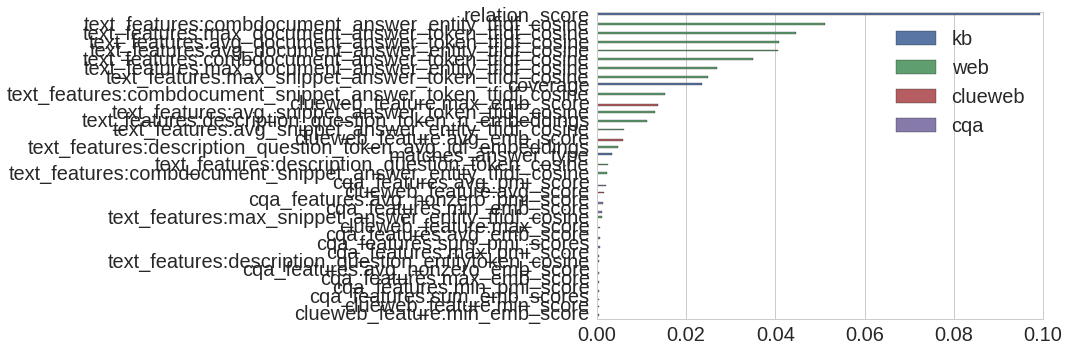
\includegraphics[width=0.8\textwidth]{img/feature_importances}
\vspace{-4mm}
\caption{A plot of Gini importances of different features of our answer ranking random forest model (features marked * are not text-based and are provided for comparison)}
\label{fig:feature_importances}
\end{figure*}

In summary, Text2KB significantly outperforms the baseline system, and each of the introduced components contributes to this improvement.
Web search results data turned out to be the most useful resource, and it significantly improves the quality by helping with question entity identification and candidate ranking.
Next, we analyze the system performance in more detail, and investigate factors for future extension.